\documentclass[a4paper,8pt]{article}
\usepackage[utf8]{inputenc}
\usepackage[english]{babel} %language
\usepackage[
backend=bibtex
]{biblatex}
\addbibresource{references.bib}
\usepackage{amssymb}
\usepackage{listings}
\usepackage{xcolor}
\usepackage{array}
\usepackage{float}
\usepackage{amsmath}

%CodeColours
\definecolor{codegreen}{rgb}{0,0.6,0}
\definecolor{codegray}{rgb}{0.5,0.5,0.5}
\definecolor{codepurple}{rgb}{0.58,0,0.82}
\definecolor{backcolour}{rgb}{0.95,0.95,0.92}
\definecolor{codeblue}{rgb}{0,0,0.80}



%Codestyle
\lstdefinestyle{mystyle}{
	backgroundcolor=\color{backcolour},   
	commentstyle=\color{codegreen},
	keywordstyle=\color{orange},
	numberstyle=\tiny\color{codegray},
	stringstyle=\color{codepurple},
	basicstyle=\ttfamily\footnotesize,
	identifierstyle=\color{codeblue},
	breakatwhitespace=false,         
	breaklines=true,                 
	captionpos=b,                    
	keepspaces=true,                 
	numbers=left,                    
	numbersep=5pt,                  
	showspaces=false,                
	showstringspaces=false,
	showtabs=false,                  
	tabsize=2,
	basicstyle=\scriptsize
}
%Set style
\lstset{style=mystyle}

%Images and similar
\usepackage{graphicx}
\graphicspath{.}

%timeline
\usepackage{tikz}
\usetikzlibrary{snakes}
\usepackage{rotating}

\title{Title}
\author{Simon dos Reis Spedsbjerg}

\newcommand{\Phases}{7 }
\newcommand{\phaseq}{Related Work}
\newcommand{\phasew}{Data Collection}
\newcommand{\phasee}{Analysis}
\newcommand{\phaser}{Design}
\newcommand{\phaset}{Implementation}
\newcommand{\phasey}{Software Evaluation}
\newcommand{\phaseu}{Evaluation}

\usepackage{biblatex}


\usepackage[acronym]{glossaries}
\newacronym{reps}{REPS}{Relational Event Prediction System}
\newacronym{gui}{GUI}{Graphical User Interface}

\begin{document}
	\maketitle
	\section{Context}
		The amount of data collected forever increases, and systems ever become more dependent on the quality of the data. Faulty time series data may damage the quality of analysis that is performed on the data, and outlier data may indicate another system is failing, or an uncommon phenomenon has occurred. As sensor values rarely are independent of other environmental variables, decrease in temperature leads to increase in power consumption for heating leads to higher heating bill. While if power consumption did not rise might indicate that the people have extra cloths on or is using another heat source. The goal is to predict future events or explain current events so the administrator of the system can proactively mitigate the event. Sensors that give of data which is abnormal might indicate need for maintenance\cite{MUKHERJEE2024102444}, a specific event, or a successful intrusion into some parts of the system\cite{MR2022103046}. Information to predict events or needs has become an interest in many sectors, Mukherjee, A\cite{MUKHERJEE2024102444} cites transport, manufacturing, water, and power, while they themselves trying to predict maintenance for container cranes. Predicting ongoing events might have high importance when it comes to cyberattacks. Gauthama et al. worked on analysing possible attack detection systems in a water treatment plant using its multipoint IOT sensory system\cite{MR2022103046}.
			
	\section{Problem}
		I define \gls{reps} as a system which attempts to predict an event based on changes to a variable and variables which it shares any form of relation with.\\
		Research Questions:
		\begin{itemize}
			\item RQ1: What is the benefit of a \gls{reps} in a system with multiple sensors?
			\item RQ2: What advantages and disadvantages does \gls{reps} have compared to state-of-the-art solutions?
		\end{itemize}
	\newpage
	\section{Approach}
		To find answers to the research questions, I propose 2 approaches: 
		\begin{itemize}
			\item \textbf{Qualitative Comparison}, using the data I will simulate a real-life system using separate computers as individual systems where my system, \gls{reps}, will try to make predictions. I will also implement other algorithms that tries to solve the same or similar problems, and make qualitative comparisons to determine whether \gls{reps} has any validity.
			\item \textbf{Digital Twin}, The second approach is to set up digital twins of systems where the \gls{reps} would be a fit and generate the data live and then compare it to state-of-the-art solutions to determine the validity of \gls{reps} system. This will require constant attention that the digital twins do not give an advantage to \gls{reps} when compared to other algorithms which solves the same problem.
		\end{itemize}
		 
		
		
	\section{Timeline}
	I intend to go into \Phases phases during this project.
		\begin{itemize}
			\item \textbf{\phaseq}, develop a clear and thorough understanding of the current state of research in anomaly detection and 'fault detection and diagnosis' by creating a systematic literature review of the subjects.
			\item \textbf{\phasew}, Collect or create relevant data depending on the results of the \phaseq \space which is relevant to the subject. As the results will be drawn on the solution's ability to handle the data, the quality of the data has a high impact on the project.
			\item \textbf{\phasee}, analyse the problem with the help of software engineering methods based on the \phaseq \space results.
			\item \textbf{\phaser}, design a theoretical solution to the problem specified in the \phasee \space phase with software engineering methods.
			\item \textbf{\phaset}, develop the project based on the results of the \phasee \space and \phaser \space using software engineering methods. This includes setup for any experimentations.
			\item \textbf{\phasey}, how well does the solution fulfil the requirements determined in the \phasee \space phase and does it implement all features which is deemed critical .
			\item \textbf{\phaseu}, verify the results from the project and check if it fulfils the hypothesis. From this, draw a conclusion.
		\end{itemize}
	
	In the following, we see the expected timeline for the project.\newline
	%Timeline
	\begin{center}
			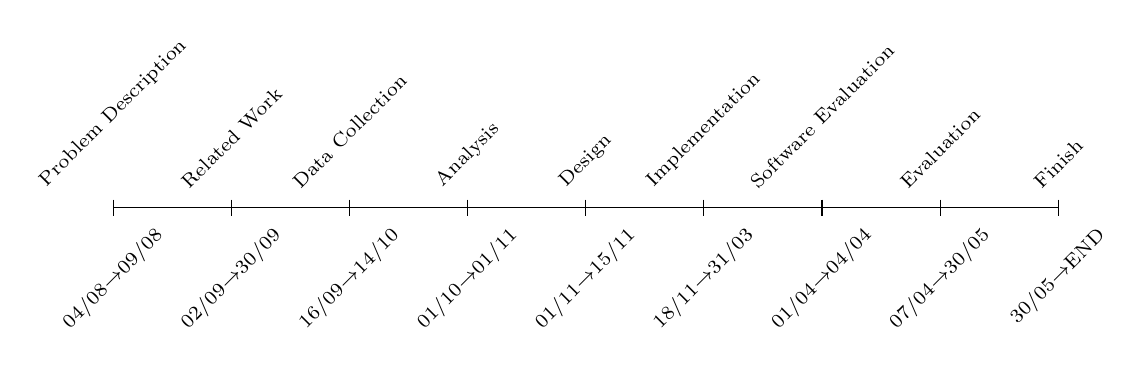
\begin{tikzpicture}
			%create the line
			\draw (-6,0) -- (6,0);
			
			%vertical lines
			\foreach \x in {-6, -4.5, -3, -1.5, 0, 1.5, 3, 4.5, 6}
			\draw (\x cm, 3pt) -- (\x cm, -3pt); %Size of the points in the timeline
			
			%draw
			\draw (-6,0) node[below=3pt] {\begin{turn}{45}\scriptsize 04/08$\rightarrow$09/08\end{turn}}
			node[above=3pt] {\scriptsize\begin{turn}{45}Problem Description\end{turn}}; %start date
			\draw (-4.5,0)
			node[below=3pt] {\begin{turn}{45}\scriptsize 02/09$\rightarrow$30/09\end{turn}}
			node[above=3pt] {\scriptsize\begin{turn}{45}\phaseq\end{turn}};
			
			\draw (-3,0)
			node[below=3pt] {\begin{turn}{45}\scriptsize 16/09$\rightarrow$14/10\end{turn}}
			node[above=3pt] {\scriptsize\begin{turn}{45}
					\phasew
			\end{turn}};
			
			\draw (-1.5,0)
			node[below=3pt] {\begin{turn}{45}\scriptsize 01/10$\rightarrow$01/11\end{turn}}
			node[above=3pt] {\scriptsize\begin{turn}{45}
					\phasee
			\end{turn}};
			
			\draw (0,0)
			node[below=3pt] {\begin{turn}{45}\scriptsize 01/11$\rightarrow$15/11\end{turn}}
			node[above=3pt] {\scriptsize\begin{turn}{45}
					\phaser
			\end{turn}};
			
			\draw (1.5,0)
			node[below=3pt] {\begin{turn}{45}\scriptsize 18/11$\rightarrow$31/03\end{turn}}
			node[above=3pt] {\scriptsize\begin{turn}{45}
					\phaset
			\end{turn}};
			
			\draw (3,0)
			node[below=3pt] {\begin{turn}{45}\scriptsize 01/04$\rightarrow$04/04\end{turn}}
			node[above=3pt] {\scriptsize\begin{turn}{45}
					\phasey
			\end{turn}};
			
			\draw (4.5,0)
			node[below=3pt] {\begin{turn}{45}\scriptsize 07/04$\rightarrow$30/05\end{turn}}
			node[above=3pt] {\scriptsize\begin{turn}{45}
					\phaseu
			\end{turn}};
			
			\draw (6,0) node[below=3pt]{\begin{turn}{45}\scriptsize 30/05$\rightarrow$END\end{turn}} node[above=3pt] {\scriptsize\begin{turn}{45} Finish \end{turn}};%end date
		\end{tikzpicture}
	\end{center}
	{\scriptsize a Gantt version exists in appendix}\\
	Every 1-4 weeks a plan will be made detailing the coming weeks' task. Each time a plan is made, the previous weeks will be documented on what went well, okay, not so well, and terribly. This is so the supervisor and I can create a perspective and course correct if need be.
	
	The plan is to hold meetings with the supervisor at least every week, an agenda will be send to the supervisor at minimum 48 hours before the meeting.

	
	\section{Preliminaries/Feasibility}
		The will have a high chance of success based on the risk analysis and as long the mitigation tactics are used.
	
		\subsection{Risk analysis}
			The risk levels are as follows, insignificant, very low, low, medium, high, very high. This is the likelihood of the risk coming true. An impact value is also set and it has the same levels as the risk levels. Mitigation is the tactic and how well it can be mitigated if the risk were to happen. All these factors will be taken into consideration throughout the project's lifetime based on the cost-benefit.
			{\scriptsize
			\begin{center}
				\begin{tabular}[!h]{|m{8em}|m{6em}|m{5em}|m{5em}|m{5em}|m{9em}|}
					\hline
					Risk Type & Description & Risk & Impact & Mitigation & Comments \\ \hline
					Missing Related work & There is not enough related work to form a proper ground for research & Insignificant & Very high & Reformulate research question & Already from the research that I have read for this topic, it is clear that there is more than enough. \\ \hline
					Unable to gather data for simulations & Either I am able to gain the data or I will have to set up some form of a digital twin. & Medium & Medium & Set up digital twins; what the twin is of will be decided after going through related work & The twin is not intended to fit perfectly with the system that I intend to implement, it is supposed to be used to decide whether it is in general a possible solution to the problem while comparing it to other solutions whose goal is to solve the same problem.\\ \hline
					Collected data or Twin is over-fitted for the implementation & Over-fitting means that it just fits too well for this specific case but will not give similar results in other similar scenarios which would fail the project. & Medium & Very High & As long as this is kept in mind throughout the project with the intention it should not fit perfectly, it should not be a problem. & The problem will most likely happen if this is forgotten about, emphasising constant thought and care about this problem. \\ \hline
					Implementation fails & The implemented code is in a state where it fails to give useful results that allow me to answer the research questions. & Very low & Very High & Implement only 'must have' requirements and scale the system down in size & In my opinion is scaleable, while scaling down will give a worse result, it will allow for the completion of the project. \\ \hline
				\end{tabular}
			\end{center}
			}
		\begin{figure}[tbp]
			\begin{center}
				\scalebox{0.7}{
					\rotatebox{90}{
						\ldots
					}
				}
			\end{center}

		\end{figure}
	\printbibliography
	\newacronym{reps}{REPS}{Relational Event Prediction System}
\newacronym{gui}{GUI}{Graphical User Interface}
	
	\section{Appendix}
	\begin{figure}[!h]
		\begin{center}
			\scalebox{0.82}{
					\rotatebox{-90}{
					\includegraphics[width=1.8\columnwidth]{Gantt}
				}
			}
		\end{center}
		\caption{Gantt Diagram over the expected task for the project}
		\label{img:Gantt}
	\end{figure}
\end{document}